\thispagestyle{empty}
\AddToShipoutPicture*{\put(0,0){%
\parbox[b][\paperheight]{\paperwidth}{%
\vfill
\centering
\refstepcounter{dummy}
\includegraphics[width=\dimen107,height=\dimen108,keepaspectratio]{img/we_want_you.jpg}%
\label{we_want_you}
\vfill
}}}
\
\pagebreak

\addchap{Grußwort}

\begin{wrapfigure}{l}{0.31\textwidth}
  \vspace{-12pt}
  \begin{centering}
    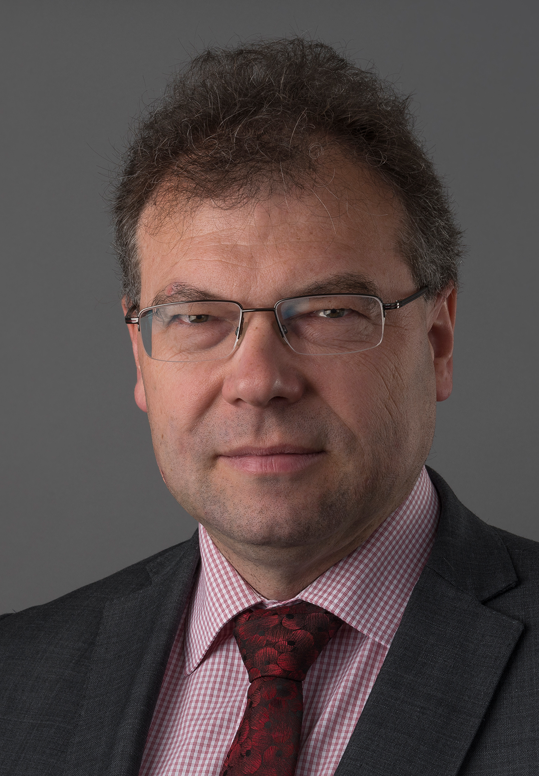
\includegraphics[width=0.3\textwidth]{img/uweassmann.png}
  \end{centering}
  \vspace{-15pt}
\end{wrapfigure}

{\fontsize{10pt}{11}\selectfont

Liebe Studierende,

herzlichen Glückwunsch zum Beginn eines der spannendsten Studien, die es gibt, an  einer der attraktivsten Informatikfakultäten Deutschlands und Europas!  Als Dekan ist es mir eine Freude, Sie herzlich an unserer Fakultät  Informatik begrüßen zu dürfen. Mit 26 Professoren, 3 Honorarprofessoren, mehr als 300 Mitarbeitern und mehr als 1600 Studenten gehört die  Fakultät zu den größten Informatikfakultäten Deutschlands mit einem der  breitesten Spektren an Studieninhalten. Um unser modernes Gebäude werden wir von vielen anderen Fakultäten beneidet, auch wenn es manchmal mit  einem Augenzwinkern als \enquote{Grünes Gewölbe} bezeichnet wird. Ich  kann Ihnen aus eigener Erfahrung versichern: man gewöhnt sich an die  Farbe. Das Gebäude bietet nicht nur Platz für die Mitarbeiter der  Fakultät, sondern verfügt auch über einen Vorlesungssaal, diverse  Seminarräume und hochwertig ausgestattete Rechner-Pools. Im Foyer  liefert das Studentencafé \ascii{} den für einen Wissenschaftsbetrieb  äußerst wichtigen Koffeinnachschub. Was unser Kunstwerk im Atrium  bedeutet, dürfen Sie gerne raten. Hinter unserem Gebäude lädt das  \enquote{Nöthnitzer Meer} zum Lernen, Chillen und Sonnen ein. Und gleich links von der Fakultät liegt unser beliebtes Sportzentrum.

Die Informatik durchdringt unsere Gesellschaft wie keine andere  Wissenschaft und beschleunigt den wissenschaftlichen Fortschritt anderer Disziplinen enorm. Marc Andreesen, der Erfinder des ersten  kommerziellen Web-Browsers \enquote{Netscape}, prägte in 2011 den Slogan \enquote{Software is eating the world}, was sagen will, dass die  Digitalisierung alle Industrien und alle Lebensbereiche verändert.  Software läuft nicht nur in Computern, sondern auch in Autos,  Flugzeugen, Wasch- und Kaffeemaschinen. Gerade im Zeitalter von Corona sieht man, wie groß der Einfluss von  Software ist. Trotz widerwärtiger Umstände konnten wir im Sommersemester 2020 mit e-learning- und Konferenzsystemen den Lehrbertrieb aufrecht erhalten - ohne diese modernen Apps hätte alles eingestellt werden müssen. Die Digitalisierung führt auch dazu, dass  Firmen händeringend nach Informatikern suchen. Unsere Fakultät kann  derzeit mit ihren Absolventen nicht einmal den Fachkräftebedarf der  Software-Industrie im Raum Dresden decken, denn sie wächst jedes Jahr um ca. 5--7\% und benötigt dazu ca. 600 neue Informatiker. Nach dem  erfolgreichen Abschluss Ihres Studiums werden Ihnen daher viele Türen  offenstehen. Herzlichen Glückwunsch zu diesen guten Aussichten!

Für  Sie, liebe Studentinnen und Studenten, beginnt mit dem Studium ein  neuer, faszinierender Lebensabschnitt, der mehr Freiheiten bietet als  die Schule vorher und das Berufsleben danach. Diese Freiheiten sollten  Sie nutzen, um sich in freier Selbstbestimmung zu bilden, Ihr Studium  selbst zu planen, Ihre Lerninhalte selbst zu vertiefen und sich selbst  Ihre Lern-Arbeit einzuteilen. Das macht Spaß -- es bringt aber auch zwei Probleme mit sich: Erstens muss man das systematische Erarbeiten von  großen Mengen an Lernstoff trainieren, und zweitens benötigt man für ein erfolgreiches Studium mehr Disziplin, als man von der Schule gewohnt  ist. Also, einige Tipps: Gehen Sie bitte regelmäßig in die Vorlesungen,  denn der Professor fasst dort für Sie die wichtigsten Inhalte des  Fachgebiets zusammen, sodass Sie schnell Wichtiges von Unwichtigem  unterscheiden können. Bereiten Sie bitte diese Kerninhalte Ihres Faches  regelmäßig nach, denn dann verankern sie sich schneller in Ihrem Kopf -- nichts ist schlimmer als eine Woche Bulimie-Lernen vor der Prüfung.  Schließlich: Erarbeiten Sie sich die Lösungen zu den Übungsaufgaben  selbstständig, denn das selbstständige Lösen von Aufgaben führt Sie  schnell zu einer höheren Stufe des Lernens und der damit verbundenen  Leistungsfähigkeit (Bloomsche Lernzielhierarchie, siehe Wikipedia). Das  erfolgreiche Herunterladen der Vorlesungsfolien oder des Skripts zur  Vorlesung trägt nur dann zum Bestehen der Prüfung bei, wenn Sie sich  auch intensiv mit den Inhalten auseinandersetzen :-) Versuchen Sie, alle Begriffe zu verstehen und zusätzlich in der Lage zu sein, sie aktiv  erklären zu können. Laden Sie sich gegenseitig zum Kaffee ins \ascii{}  ein und erklären Sie sich dabei, was in der letzten Vorlesung behandelt  worden ist.  Das verbessert nicht nur den Studienerfolg, sondern macht  auch viel mehr Spaß. (Das habe auch ich in meinem Studium so erlebt.)  Und wenn Sie trotzdem im Studium auf Probleme stoßen, stehen Ihnen viele Anlaufstellen zur Verfügung: Studienberater, Mitglieder des  Fachschaftsrates, Übungsgruppenleiter und selbstverständlich auch alle  Professoren, die für Sie Sprechstunden anbieten, die Sie nutzen sollten, insbesondere zu einem Check vor Prüfungen.

Am Ende meines Grußwortes möchte ich mich ganz herzlich beim  Fachschaftsrat für das große Engagement in der Fakultät und insbesondere für die Durchführung der Erstsemestereinführung bedanken. Die Fakultät  lebt vom Engagement aller Mitglieder, insbesondere ihrer Studenten. Im  Gegenzug bekommen Sie von uns ein vielfältiges Angebot, und das ohne  Studiengebühren. Warum sollten Sie also Ihr Studium nicht als einen  \enquote{ungewöhnlicherweise kostenlosen Supermarkt} betrachten, den Sie durch den \enquote{Einkaufswagen Ihres Lernens ausräumen}, um später im Leben erfolgreich sein zu können? Es liegen viele spannende Themen vor  uns. Gestalten Sie also mit uns die Zukunft der Informatik und mit ihr  die Gesellschaft. WE WANT YOU FOR YOUR FUTURE\@!

\textit{Uwe Aßmann,\\
Dekan der Fakultät Informatik}
